\documentclass{beamer}
% \usepackage{animate}
\usepackage{multimedia}
\usepackage[english,russian]{babel}

\usepackage{pgfpages}
\setbeameroption{show notes on second screen}
%https://tug.ctan.org/macros/latex/contrib/beamer/doc/beameruserguide.pdf

\usepackage[T2A]{fontenc}
\usepackage[utf8]{inputenc}

\setbeamertemplate{caption}[numbered]

\usetheme{CambridgeUS}
\usecolortheme{dolphin}


\title[Memory Vulkan API]{Память в Vulkan API}
\author[Быковских Д.А.]{Быковских Дмитрий Александрович}
\date{05.10.2024}

\begin{document}
	\begin{frame}
		\titlepage
	\end{frame}
	%\section{Обзор}
	\begin{frame}{Введение}

		\begin{itemize}
			\item 
			Рассмотреть объекты Vulkan API
			\item
			Рассмотреть модель графического конвейера Vulkan API
			\item
			Далее по слайдам....
		\end{itemize}

		\note{
			Для правильного выбора и настройки ресурсов, используемых в шейдерах, следует понимать, какие типы данных существуют, где их следует хранить, как использовать/связывать и т.д.
			
			Например, вершинные атрибуты (позиция, цвет, нормали и т.д.), 
			
			буферы, используемые для хранения общей информации о моделях,

			изображения (сэмплеры) с целью быстрого достоптупа к изображению, 

			и т.д.
		}
	\end{frame}
	
	\begin{frame}{Иерархия памяти современной графической карты}
		\begin{figure}
			\href{https://www.researchgate.net/figure/A-schematic-of-the-memory-hierarchy-of-the-Nvidia-Fermi-architecture-with-the-peak_fig4_51927898}{
				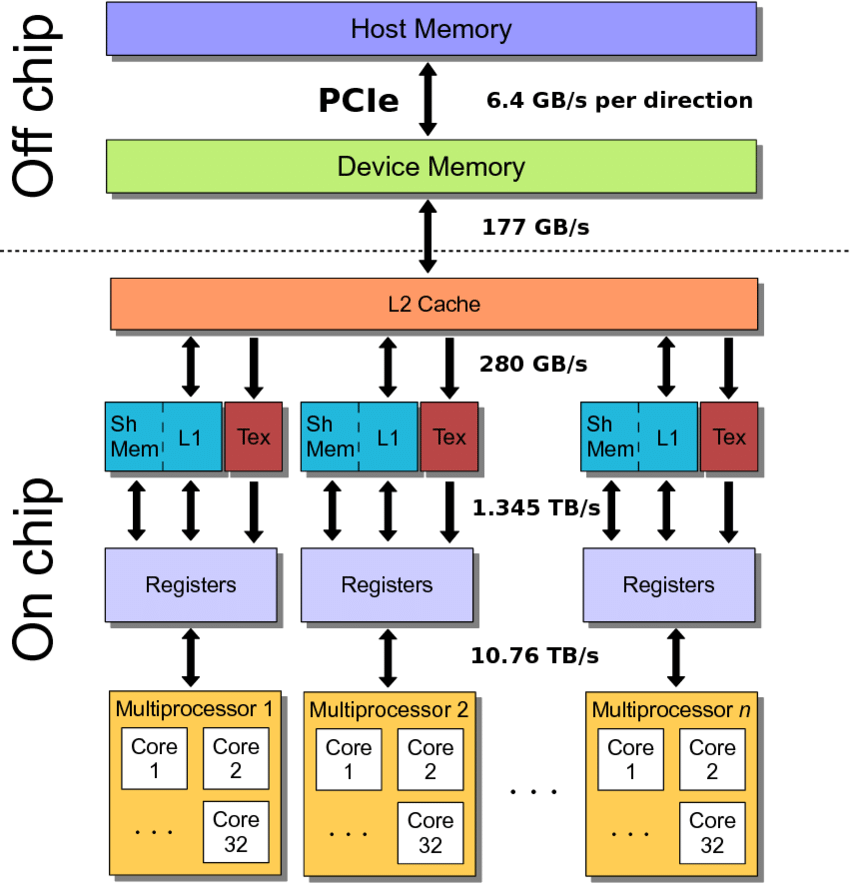
\includegraphics[width=0.5\textwidth]{images/Memory-hierarchy-of-the-Nvidia-Fermi-architecture.png}}
			\caption {Схема иерархии памяти архитектуры Nvidia Fermi}
		\end{figure}
	
		\note {
	
	
		}
	\end{frame}


	\begin{frame}{Информация о типах памяти}
		Memory heaps (кучи) делятся на категории
		\begin{itemize}
			\item 
			Device local and host invisible 
			\item
			Device local and host visible
			\item 
			Host local and device visible 
		\end{itemize}
		Примечание:
		Первый из перечисленных типов памяти обладает самой высокой пропускной способностью.
		(см. Vulkan Hardware Capability Viewer)

\note{
	\scriptsize
	При разработке программ следует понимать следующие типы памяти
	\begin{itemize}
		\item 
		Стек (stack) --- это структура данных, организованная по принципу LIFO (Last In, First Out — последним пришёл, первым ушёл). 
		Особенность его использования связана с вызовом функций.
		В первую очередь стек хранит адрес возврата и локальные переменные функций. 
	 	Каждая новая вызванная функция добавляется в стек, а после завершения работы функции стек «сворачивается» обратно.
		\item
		Куча (heap) --- это область динамической памяти, управляемая программой вручную. 
		Она используется для хранения объектов, которые создаются в процессе выполнения программы, когда невозможно заранее предугадать размер памяти, который потребуется.
		Доступ к элементам в куче происходит напрямую через указатели или ссылки.
		Управление памятью в куче выполняется самостоятельно (т.е. нет сборщика мусора, может приводить к утечке).
	\end{itemize}
	
	Замечания:

	1. Операции со стеком, как правило, быстрее, поскольку работают с последним добавленным элементом, тогда как в куче требуется больше времени для поиска и управления памятью.

	2. Стек имеет ограничение на количество выделяемой памяти, в то время, как куча ограничена размерами физической памяти.

}
	\end{frame}

	\begin{frame}{Информация о свойствах памяти}
		Поддерживаемые свойства (VkMemoryPropertyFlags) представленных типов памяти (Host и Device)
		{ \scriptsize
		\begin{itemize}
			\item 
			$DEVICE\_LOCAL\_BIT$

			Память графической карты.
			\item
			$HOST\_VISIBLE\_BIT$
			
			Память, которая доступна для доступа CPU через mapped pointer (после вызова vkMapMemory). Доступ осуществляется так, будто CPU имеет дело с системной памятью (возможен механизм, который позволяет CPU обращаться непосредственно к памяти видеокарты).
			\item 
			$HOST\_COHERENT\_BIT$
			
			Означает, что не требуется вызов функции vkFlushMappedMemoryRanges для того, чтобы сделать изменения в памяти, сделанный CPU, видимыми для GPU и не требуется вызов функции vkInvalidateMappedMemoryRanges для того, чтобы сделать изменения в памяти, сделанные GPU, видимыми для CPU.
			\item 
			$HOST\_CACHED\_BIT$

			Чтение CPU из такой памяти более эффективно, однако такая память не всегда является host coherent.
			\item 
			$LAZILY\_ALLOCATED\_BIT $
			
			Память для данного типа ресурса не будет выделена до тех пор, пока она не станет действительно необходимой.
		\end{itemize}
		}
\note{ \scriptsize
	\if 0
	Примечание
	Следует отметить, что GPU может иметь доступ и к системной памяти через механизм DMA, хотя это и менее эффективно.

	DMA (Direct Memory Access, прямой доступ к памяти) — это механизм, позволяющий устройствам (таким как GPU, сетевые карты, дисковые контроллеры и другие периферийные устройства) обмениваться данными с системной памятью (RAM) напрямую, минуя центральный процессор (CPU). Это повышает эффективность передачи данных, так как освобождает CPU от необходимости контролировать каждую операцию чтения или записи.
	Тип памяти с только одним флагом $DEVICE\_LOCAL\_BIT$ лучше всего подходит для данных, хранящихся в памяти GPU постоянно и используемых только GPU, таких как вершинные и индексные буферы, текстуры и т.п.
	
	Комбинации флагов $HOST\_VISIBLE\_BIT$ и $HOST\_COHERENT\_BIT$ обычно соответствует некоторая область памяти (обычно фиксированного размера), в которую CPU может писать на каждом кадре. Этот тип лучше всего подходит для постоянно изменяющихся данных, таких как uniform-буферы и динамические вершинные буферы.
	
	Комбинация $HOST\_VISIBLE\_BIT$  и $HOST\_COHERENT\_BIT$ обычно обозначает память CPU, которая непосредственно видна GPU. Если нет памяти предыдущего типа, то этот тип лучше всего подходит для постоянно изменяющихся данных.
	\fi
	
	Некоторые примеры:
	
	1. Область памяти с только одним флагом $DEVICE\_LOCAL\_BIT$ используется для данных, которые будут использоваться исключительно GPU (вершинные буферы, текстуры и т.п.). Такой способ обеспечивает высокую производительность для GPU-доступа.
	Если необходимо, то для передачи данных используются промежуточные буферы с флагами $HOST\_VISIBLE\_BIT$  и $HOST\_COHERENT\_BIT$.

	2. Область памяти с флагами $HOST\_VISIBLE\_BIT$ и $HOST\_COHERENT\_BIT$ подходит для данных, которые будут часто обновляться CPU и передаваться GPU (uniform-буферы, динамические буферы), при этом имеет легкий доступ CPU без необходимости явной синхронизации.
	
	}
		
	\end{frame}

	\if 0
	\begin{frame}{Процесс управления ресурсами}
		Этапы 
		\begin{itemize}
			\item 
			Выбор объекта ресурсов (как правило, это буфер или изображение)
			\item
			Выделение блоков памяти (управление через логические адреса; частое выделение --- дорогостоящий процесс)
			\item 
			Разреженная память (данные загружаются по мере необходимости)
			\item 
			Промежуточный буфер (используется для передачи данных)
			\item 
			Передача данных осуществляется асинхронно.
			
		\end{itemize}
\note{
	}
	\end{frame}
	\fi

	\begin{frame}{Процесс управления ресурсами}
		Этапы работы
		\begin{itemize}
			\item 
			Создание объекта с данными
			(например, загрузка моделей)
			\item
			Запрос подходящего типа памяти и создание типа объекта 
			(например, буфер или изображение) 
			\item 
			Установка требований к выделению памяти
			\item 
			Выделение области памяти и сохранение данных в него
			(возможно, потребуется промежуточный буфер)
			\item 
			Связывание область памяти с данными с типом созданного объекта
			(выполняется через дескрипторы)
		\end{itemize}
\note{
Набор дескрипторов --- интерфейс, связывающий ресурсы (буферы, изображения и т.д.) и шейдеры.

Пул дескрипторов, позволяет сохранить такие наборы, которые можно использовать в дальнейшем.
	}
	\end{frame}

\if 0
\begin{columns}
	
	\begin{column}{0.5\textwidth}
		\begin{itemize}
			\item
			
		\end{itemize}
	\end{column}
	\begin{column}{0.5\textwidth}
		\begin{itemize}
			\item
		\end{itemize}
	\end{column}
	
\end{columns}
\fi
\end{frame}
	
\end{document}
